\documentclass[12pt]{ctexart}
\usepackage[english]{babel}
\usepackage{natbib}
\usepackage{url}
\usepackage[utf8x]{inputenc}
\usepackage{amsmath}
\usepackage{graphicx}
\usepackage{float}
\usepackage{subfigure}
\graphicspath{{images/}}
\usepackage{parskip}
\usepackage{fancyhdr}
\usepackage{vmargin}
\usepackage{booktabs}
\usepackage{indentfirst}
\setmarginsrb{3 cm}{2.5 cm}{3 cm}{2.5 cm}{1 cm}{1.5 cm}{1 cm}{1.5 cm}
\setlength{\parindent}{2em}

\title{Research on heat transfer formula}								% Title
\author{\emph{Bi qiuyu}}								% Author
\date{\today}											% Date

\makeatletter
\let\thetitle\@title
\let\theauthor\@author
\let\thedate\@date
\makeatother

\pagestyle{fancy}
\fancyhf{}
\rhead{\theauthor}
\lhead{\thetitle}
\cfoot{\thepage}

\begin{document}

%%%%%%%%%%%%%%%%%%%%%%%%%%%%%%%%%%%%%%%%%%%%%%%%%%%%%%%%%%%%%%%%%%%%%%%%%%%%%%%%%%%%%%%%%

\begin{titlepage}
	\centering
    \vspace*{0.5 cm}
    
\includegraphics[scale = 0.2]{NJU.jpg}\\[1.0 cm]	% University Logo
    \textsc{\LARGE Nanjing University}\\[2.0 cm]	% University Name
    \textsc{\large 24020010B}\\[0.5 cm]				% Course Code
	\textsc{\large University Physics \uppercase\expandafter{\romannumeral2}}\\[0.5 cm]				% Course Name
	\rule{\linewidth}{0.2 mm} \\[0.4 cm]
    {\huge \bfseries \thetitle}\\
	\rule{\linewidth}{0.2 mm} \\[1.5 cm]
	
	\begin{minipage}{0.4\textwidth}
		\begin{flushleft} \large
			\emph{Author:}\\
			\theauthor
			\end{flushleft}
			\end{minipage}
			\begin{minipage}{0.4\textwidth}
			\begin{flushright} \large
                \emph{Student Number:} \\
			171860624\\									% Your Student Number
                \emph{Department:} \\
                \emph{Computer Science}
		\end{flushright}
	\end{minipage}\\[2 cm]
	
	{\large \thedate}\\[2 cm]
 
	\vfill
	
\end{titlepage}

%%%%%%%%%%%%%%%%%%%%%%%%%%%%%%%%%%%%%%%%%%%%%%%%%%%%%%%%%%%%%%%%%%%%%%%%%%%%%%%%%%%%%%%%%

\tableofcontents
\pagebreak

%%%%%%%%%%%%%%%%%%%%%%%%%%%%%%%%%%%%%%%%%%%%%%%%%%%%%%%%%%%%%%%%%%%%%%%%%%%%%%%%%%%%%%%%%

\section{Abstract}
This paper mainly uses thermodynamic knowledge (including Fourier's law, etc.) and computer dynamic programming algorithms to study the transfer of heat over time and space in multilayer media.\\
\indent $\textbf{Keywords}$:Fourier's law; plane wall stable heat conduction; dynamic programming; micro-element method
\section{Introduction}
\indent 
When working in a high temperature environment, people need to wear special clothing to avoid burns. Special clothing is usually composed of three layers of fabric material, which are recorded as layers I, II and III. The layer I is in contact with the external environment, and there is a gap between the layer III and the skin. This space is recorded as the IV layer. In order to design special clothing, the dummy whose body temperature is controlled at $37^{o}$C is placed in the high temperature environment of the laboratory to measure the temperature outside the skin of the dummy. In order to reduce the development cost and shorten the development cycle, please use the mathematical model to determine the temperature change outside the skin of the dummy,
and solve the following problems: the ambient temperature is $75^{o}$C, the II layer thickness is 6 mm, and the IV layer thickness is 5 mm. An experiment was conducted with a working time of 90 minutes, and the temperature outside the skin of the dummy was measured. Establish a mathematical model and calculate the temperature distribution.
\section{Special Description}
In this question I understand the “temperature distribution” that needs to be solved as the temperature distribution when the system S reaches dynamic equilibrium.
In the construction of the model, I only consider heat transfer heat transfer, regardless of other forms of heat transfer (such as heat radiation, heat convection), and the heat transfer between different protective layers of the protective clothing is simplified to a single layer of planar wall stability. The heat conduction, that is, the thermal conductivity rate $\phi$, the heat transfer area $A$, and the thermal conductivity $\lambda$ are constant and do not change with time and temperature, so the function of temperature with respect to the $x$ coordinate value is a linear function in the same material.
\section{Description of Symbol}

\begin{center}
\begin{tabular}{|c|c|}
\toprule
Symbol & Meaning\\
\midrule
$\xi{0}$ & Space in a high temperature environment\\
\midrule
$\xi{1}$ & Space formed by the first layer of protective clothing\\
\midrule
$\xi{2}$ & Space formed by the second layer of protective clothing\\
\midrule
$\xi{3}$ & Space formed by the third layer of protective clothing\\
\midrule
$\xi{4}$ & Space formed by the fourth layer of protective clothing\\
\midrule
$\xi{5}$ & Space inside the dummy\\
\bottomrule
\end{tabular}
\end{center}

\section{Modeling}
According to the measured data of the outside temperature of the dummy skin over time, I use MATLAB to plot the temperature-time curve outside the skin of the dummy as follows:\\
\begin{figure}[H]
\centering
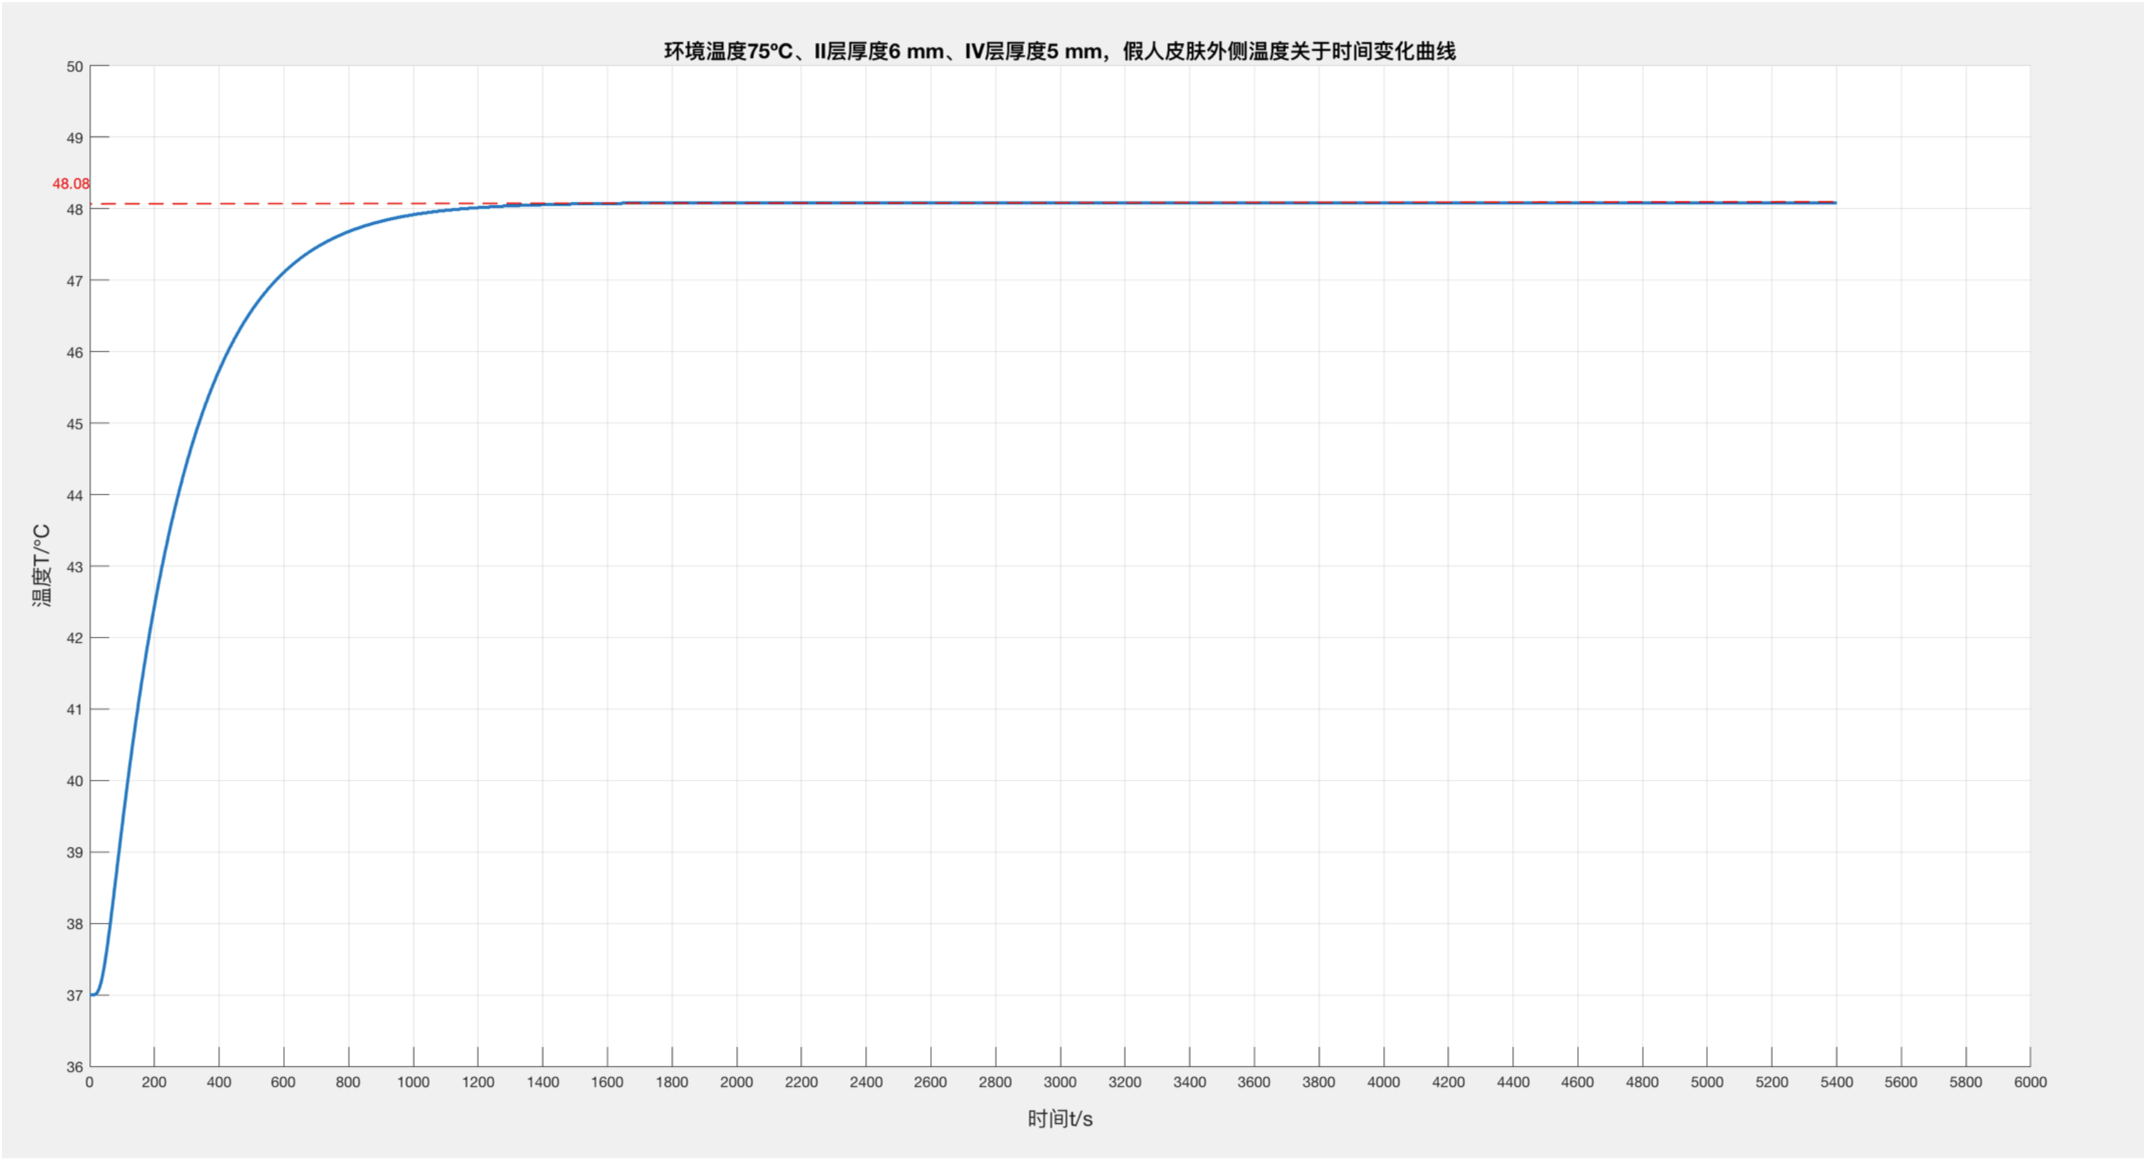
\includegraphics[width=0.8\textwidth]{1.png}
\caption{Changes of temperate according to time}
% \label{Fig 1}
\end{figure}
From the figure, we can see that the temperature outside the skin of the dummy tends to be stable with time ($T_f$ = $48.08^{o}$C). After that, the lateral stability of the dummy's skin no longer rises. It is known that the temperature inside the dummy is $37^{o}$C, the skin. After the outside temperature reached a stable state, it was maintained at $48.08^{o}$C. At this time, the heat in the high temperature environment is continuously transmitted to the dummy through the protective clothing, and the device that maintains the constant temperature of $37^{o}C$ in the dummy can continuously absorb the heat, so that the entire system $S$ reaches a dynamic equilibrium state, and the temperature is maintained everywhere stable.\\
\indent It is known that the experimental ambient temperature is constant at $75^{o}$C, the body temperature of the dummy is constant at $37^{o}C$, and the outer skin temperature is finally stabilized at $48.08^{o}C$. I will environment $\xi(T_0 , x)$-I layer $\xi(T_1 , x)$-II layer $\xi(T_2 , x)$-III layer $\xi(T_3 , x)$- IV layer $\xi(T_4 , x)$-dummy $\xi(T_5 , x)$ is regarded as a $\xi_{0} $, $\xi _1$ , $\xi_2$, $\xi_3$ , $\xi_4$ , $\xi_5$ The system $S$ composed of six regions is denoted as $S(\xi_0 , \xi_1 , \xi_2 , \xi_3 , \xi_4 , \xi_5 )$.\\

I first abstract the six regions of the system $S$ into a closed rectangle, with a point on the boundary between $\xi_{1}$ and $\xi_{2}$ as the origin, a positive direction to the right in the $x$-axis, and a plane in the positive direction of the $y$-axis. And build model 1.0, as shown below. Each region $\xi_{i} (i = 0, 1, 2, 3, 4)$ is mapped to the $x$-axis and is a left-right-closed interval. The interval length $\Delta x_{i}$ is the thickness $\delta_{i}$ of the material corresponding to the region that is $\Delta x_{i} = \delta_{i}$ .

\begin{figure}[H]
\centering
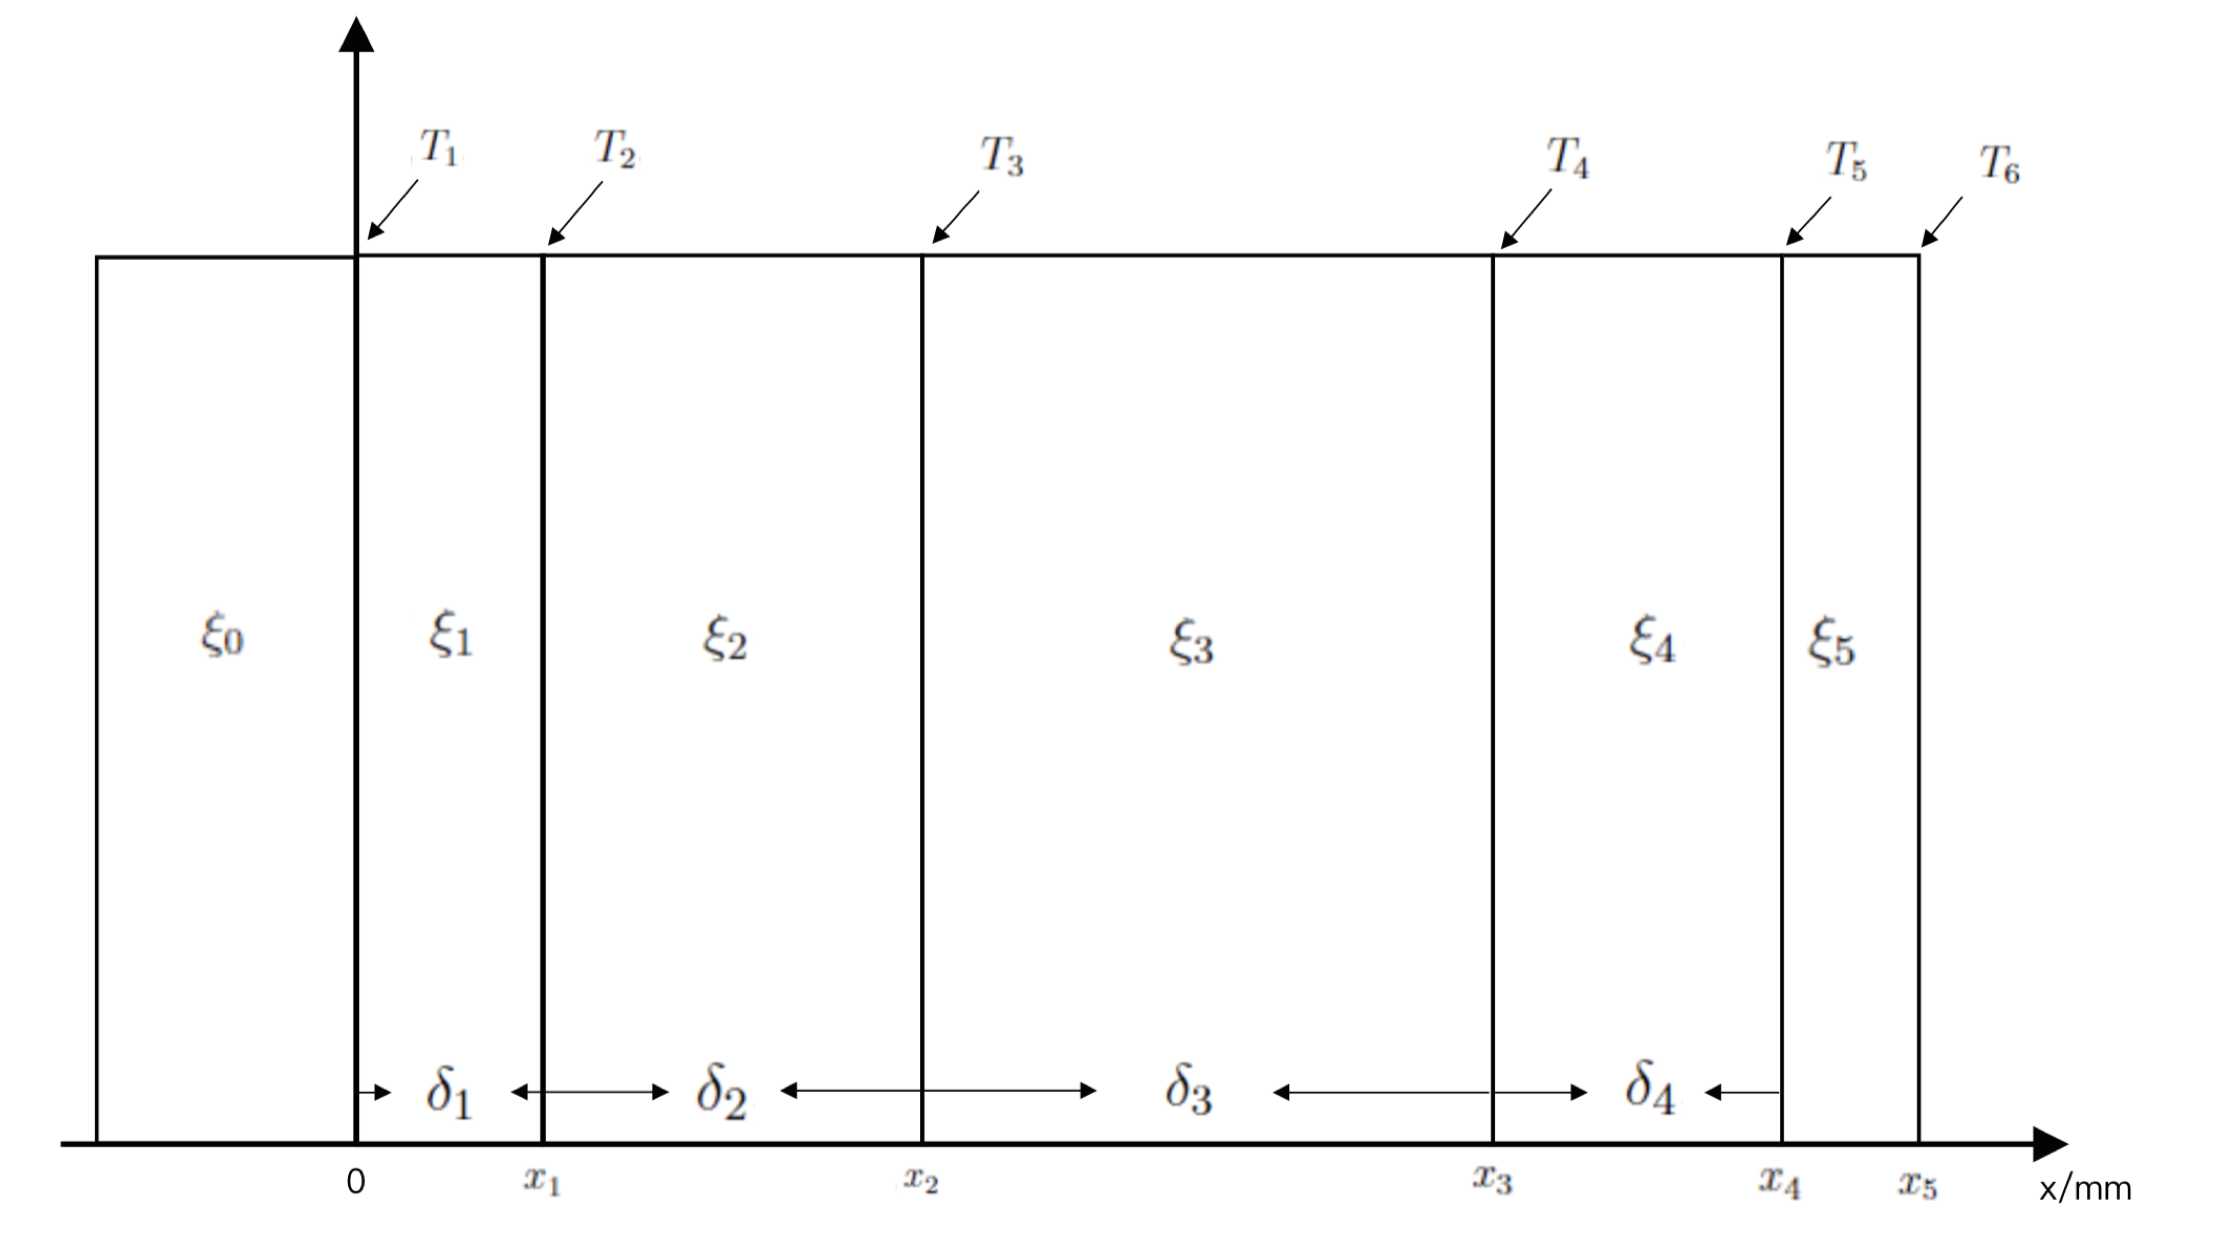
\includegraphics[width=0.8\textwidth]{2.png}
\caption{System $S$}
% \label{Fig 1}
\end{figure}
In this model, all points with the same $x$ coordinate value have the same temperature $T$, and when $x < 0$, $x \in \xi_{0}$, $T_1 \equiv 75^{o}C$; when $x = x _5$, $T_6 \equiv 37^{o}C$; After reaching steady state, $x = x_4$ at $T_5 = 48.08^{o}C$.
\section{Temperature Distribution}
In the construction of the model, I only consider heat transfer heat transfer, regardless of other forms of heat transfer (such as heat radiation, heat convection), and the heat transfer between different protective layers of the protective clothing is simplified to a single layer of planar wall stable heat conduction, ie The thermal conductivity rate $\phi$, the heat transfer area $A$, and the thermal conductivity $\lambda$ are constant and do not change with time or temperature.\\
\indent According to the Fourier law expression\cite{volz1996transient}:
\[\phi = -\lambda A\frac{dT}{dx}\]
\indent Integrate it I get:\\
\[\phi = \lambda A\frac{T_{1}-T_{2}}{\delta}\]
\indent According to the above formula, the following equation can be obtained\cite{li2004fourier}:\\
    \[\xi_1 : \phi_{1} = \frac{\lambda_{1}}{\delta_{1}}\cdot A_{1}(T_{1f}-T_{2f})\]
    \[\xi_2 : \phi_{2} = \frac{\lambda_{2}}{\delta_{2}}\cdot A_{2}(T_{2f}-T_{3f})\]
    \[\xi_3 : \phi_{3} = \frac{\lambda_{3}}{\delta_{3}}\cdot A_{3}(T_{3f}-T_{4f})\]
    \[\xi_4 : \phi_{4} = \frac{\lambda_{4}}{\delta_{4}}\cdot A_{4}(T_{4f}-T_{5f})\]
\indent $\textbf{i.e.}$\\
    \[\Delta T_{1} = T_{1f}-T_{2f}= \frac{\phi_{1}}{A_{1}}\cdot \frac{\delta_{1}}{\lambda_{1}}\]
    \[\Delta T_{2} = T_{2f}-T_{3f}= \frac{\phi_{2}}{A_{2}}\cdot \frac{\delta_{2}}{\lambda_{2}}\]
    \[\Delta T_{3} = T_{3f}-T_{4f}= \frac{\phi_{3}}{A_{3}}\cdot \frac{\delta_{3}}{\lambda_{3}}\]
    \[\Delta T_{4} = T_{4f}-T_{5f}= \frac{\phi_{4}}{A_{4}}\cdot \frac{\delta_{4}}{\lambda_{4}}\]
\indent And because S is steady state, I have a relationship:\\
    \[\phi_{1} = \phi_{2} = \phi_{3} = \phi_{4}\]
    \[A_{1} = A_{2} = A_{3} = A_{4}\]
\indent $\textbf{s.t.}$\\
    \[\frac{\lambda_{1}}{\delta_{1}}(T_{1f}-T_{2f}) = \frac{\lambda_{2}}{\delta_{2}}(T_{2f}-T_{3f}) = \frac{\lambda_{3}}{\delta_{3}}(T_{3f}-T_{4f}) = \frac{\lambda_{4}}{\delta_{4}}(T_{4f}-T_{5f})\]
\indent in expression:\\
\begin{center}
\begin{tabular}{|c|c|c|c|}
\toprule
    i & $\lambda_{i}$ & $\delta_{i}$ & $T_{if}$\\
\midrule
    1 & 0.083 & $6.0\times 10^{-4}$ & 75.00\\
\midrule
    2 & 0.370 & $6.0\times 10^{-3}$ & $T_{2f}$\\
\midrule
    3 & 0.045 & $3.6\times 10^{-3}$ & $T_{3f}$\\
\midrule
    4 & 0.028 & $5.0\times 10^{-3}$ & $T_{4f}$\\
\midrule
    5 & & & 48.08\\
\midrule
\bottomrule
\end{tabular}
\end{center}
\indent Bring known data into the equation, I get:
\[T_{2f} = 74.30^{o}C\]
\[T_{3f} = 72.75^{o}C\]
\[T_{4f} = 65.10^{o}C\]
\indent $x\in \xi_{i},(i=1,2,3,4)$, $\xi_{i}(T)$ is a linear continuous function of $x$. The Cartesian coordinate system is established with the left boundary of $\xi_{1}$ as the origin, the positive direction of the $x$-axis in the right direction, and the positive direction of the $T$-axis in the upward direction. According to the above solution, using MATLAB to find that the expressions of $\Omega(T) = (\xi_1 (T), \xi_2 (T), \xi_3 (T), \xi_4 (T))$ are:\\
\[
\Omega(T)=
\left\{
    \begin{array}{rcl}
        \xi_{1}(T) = 75.00 - \frac{7003}{6}x,       &   & {x\in [0, 6\times 10^{-4})}\\
        \xi_{2}(T) = 74.45 - \frac{15521}{60}x,     &   & {x\in (6\times 10^{-4}, 6.6\times 10^{-3}]}\\
        \xi_{3}(T) = 86.78 - \frac{76567}{36}x,     &   & {x\in (6.6\times 10^{-3}, 1.02\times 10^{-2}]}\\
    \xi_{4}(T) = 99.96 - \frac{170909}{50}x,    &   & {x\in (1.02\times 10^{-2}, 1.52\times 10^{-2}]}\\
    \end{array}
\right.
\]
\indent By combining the $\Omega(T)$ expression and the model, I can get the temperature distribution when the system $S$ reaches the dynamic equilibrium. The distribution curve of the temperature $T$ with $x$ is as follows:
\begin{figure}[H]
\centering
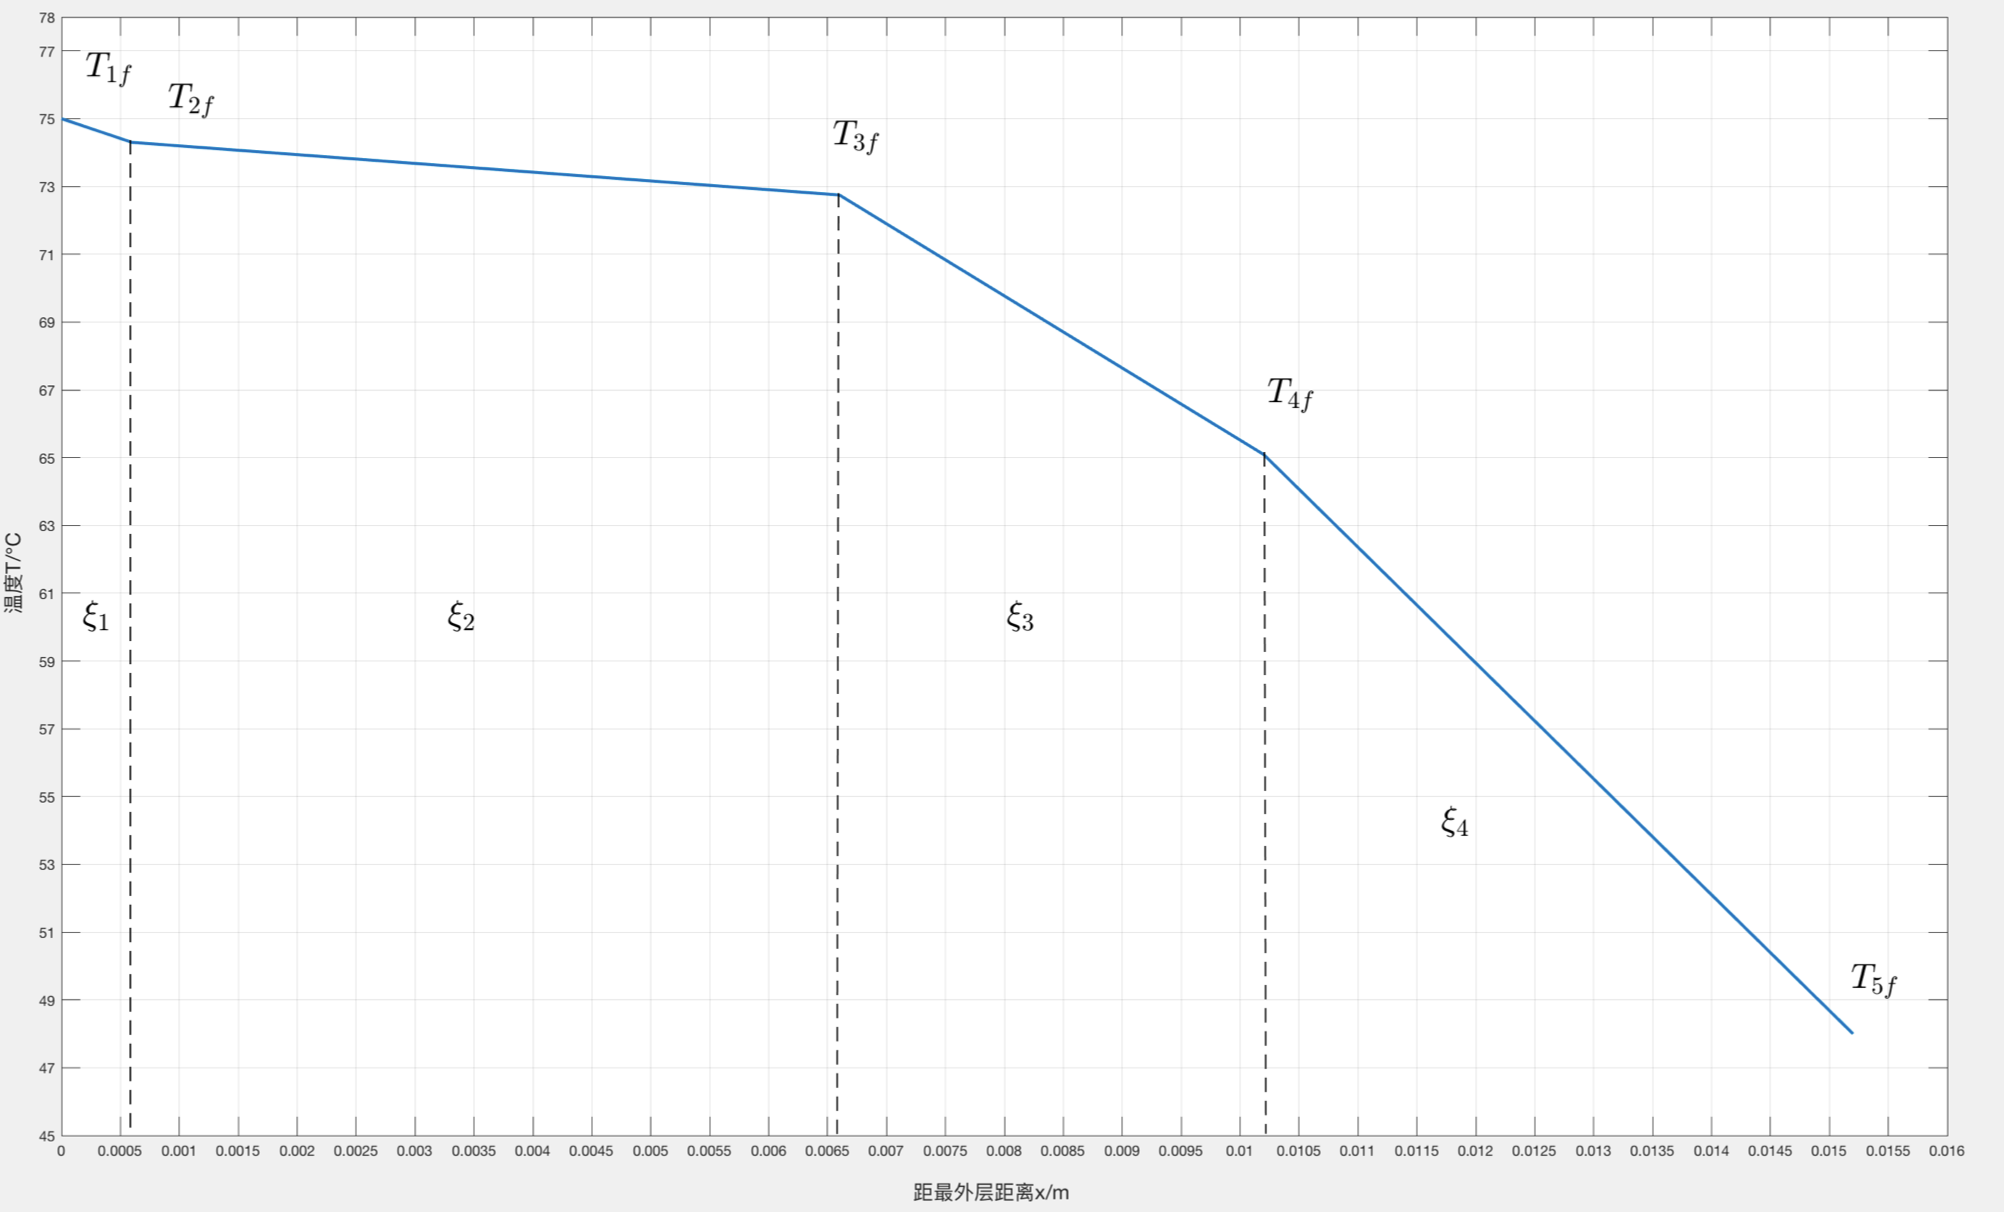
\includegraphics[width=0.8\textwidth]{3.png}
\caption{Temperature distribution when system $S$ reaches dynamic equilibrium}
% \label{Fig 1}
\end{figure}


\section{Dynamic Programming}
\indent Dynamic programming is one way to solve the optimization problem of multi-stage problem process. The basic content is: properly select the state variables, decision variables to define the optimal index function, and decompose the problem to be solved into a plurality of interrelated stages with a chain structure, that is, decomposed into multiple sub-problems $P_i (1 \leq i \leq n)$ is denoted as $P = P_1 + P_2 + \cdots + P_n$. For a given phase state, the optimal solution $P_k max$ of these subproblems $P_k$ is solved first, then according to each $P_{k}$ The solution of $P_{k}max$ is to solve the optimal solution $Pmax$ of $P$. That is, $Pmax = P_1 max + P_2 max + \cdots + P_n max$\cite{sakoe1978dynamic}.
It is said that the solution process of each $P_k max$ is related to time $t$, and the solution process satisfies the optimization principle\cite{bertsekas2005dynamic}.\\
\indent Assume that the initial temperatures of $\xi_2 , \xi_3 , \xi_4 , \xi_5$ are both $37^{o}C$, ie $T_{2i} = T_{3i} = T_{4i} = T_{5i} = 37^{o}C$. Suppose that at $t_k$ , I know the temperature
The specific value of $T_i (i = 1, 2, 3, 4, 5, 6)$ (that is, the state in the dynamic programming algorithm, that is, the state in $P_k$ is $S_k$ ), and the heat flowing into $\xi_i$ is $Q_i$ (Because it involves the heat absorption of human skin, I abstract people into another material, assuming human thermal conductivity is $\lambda_5$ ), I can get:
\[Q_{1} = \phi_{1}\cdot \Delta t = \frac{A_{1}\lambda_{1}(T_1-T_2)}{\delta_{1}}\cdot \Delta t\]
\[Q_{2} = \phi_{2}\cdot \Delta t = \frac{A_{2}\lambda_{2}(T_2-T_3)}{\delta_{2}}\cdot \Delta t\]
\[Q_{3} = \phi_{3}\cdot \Delta t = \frac{A_{3}\lambda_{3}(T_3-T_4)}{\delta_{3}}\cdot \Delta t\]
\[Q_{4} = \phi_{4}\cdot \Delta t = \frac{A_{4}\lambda_{4}(T_4-T_5)}{\delta_{4}}\cdot \Delta t\]
\indent Also by the formula\cite{callen1998thermodynamics}:
\[q_{i} = Q_{i} - Q_{i+1}\]
\[\Delta T_{i} = \frac{Q_{i}}{c_{i}\cdot m_{i}}\]
\[m_{i} = \rho_{i}V_{i} = \rho_{i}\cdot \delta_{i}\cdot A_{i}\]
\[A_{1} = A_{2} = A_{3} = A_{4} = A_{5}\]
\indent$\textbf{s.t.}$
\[\Delta T_{1} = (\frac{\lambda_{1}(T_{1}-T_{2})}{\delta_{1}} - \frac{\lambda_{2}(T_{2}-T_{3})}{\delta_{2}})\cdot\frac{\Delta_{t}}{\rho_{1}\cdot\delta_{1}\cdot c_{1}}\]
\[\Delta T_{2} = (\frac{\lambda_{2}(T_{2}-T_{3})}{\delta_{2}} - \frac{\lambda_{3}(T_{3}-T_{4})}{\delta_{3}})\cdot\frac{\Delta_{t}}{\rho_{2}\cdot\delta_{2}\cdot c_{2}}\]
\[\Delta T_{3} = (\frac{\lambda_{3}(T_{3}-T_{4})}{\delta_{3}} - \frac{\lambda_{4}(T_{4}-T_{5})}{\delta_{4}})\cdot\frac{\Delta_{t}}{\rho_{3}\cdot\delta_{3}\cdot c_{3}}\]
\[\Delta T_{4} = (\frac{\lambda_{4}(T_{4}-T_{5})}{\delta_{4}} - \frac{\lambda_{5}(T_{5}-T_{6})}{\delta_{5}})\cdot\frac{\Delta_{t}}{\rho_{4}\cdot\delta_{4}\cdot c_{4}}\]
\indent I take the initial temperatures $T_{1i} , T_{2i} , T_{3i} , T_{4i} , T_{5i} , \rho , c , \lambda_{1} , \delta_{1} , \delta_{3} , \delta_{4} $as the state variables and the required $\delta_{2}$ as the decision variables. The derived physical formula is the state transition equation, with $0.6 \leq \delta_{2} \leq 25mm (\Delta \delta = 0.01)$, the working time is 60min, the outer skin temperature does not exceed $47^{o}C$, and the time exceeding $44^{o}C$ is less than 5min as conditions for dynamic planning. Solving with computer\cite{buchanan1962calculus} and compare with the known data, I get the following graph:
I bring the condition parameters into the algorithm of dynamic programming.The curve obtained by comparing the curve of the outside temperature of the dummy skin with time and the original data is shown in the following figure:
\begin{figure}[H]
\centering
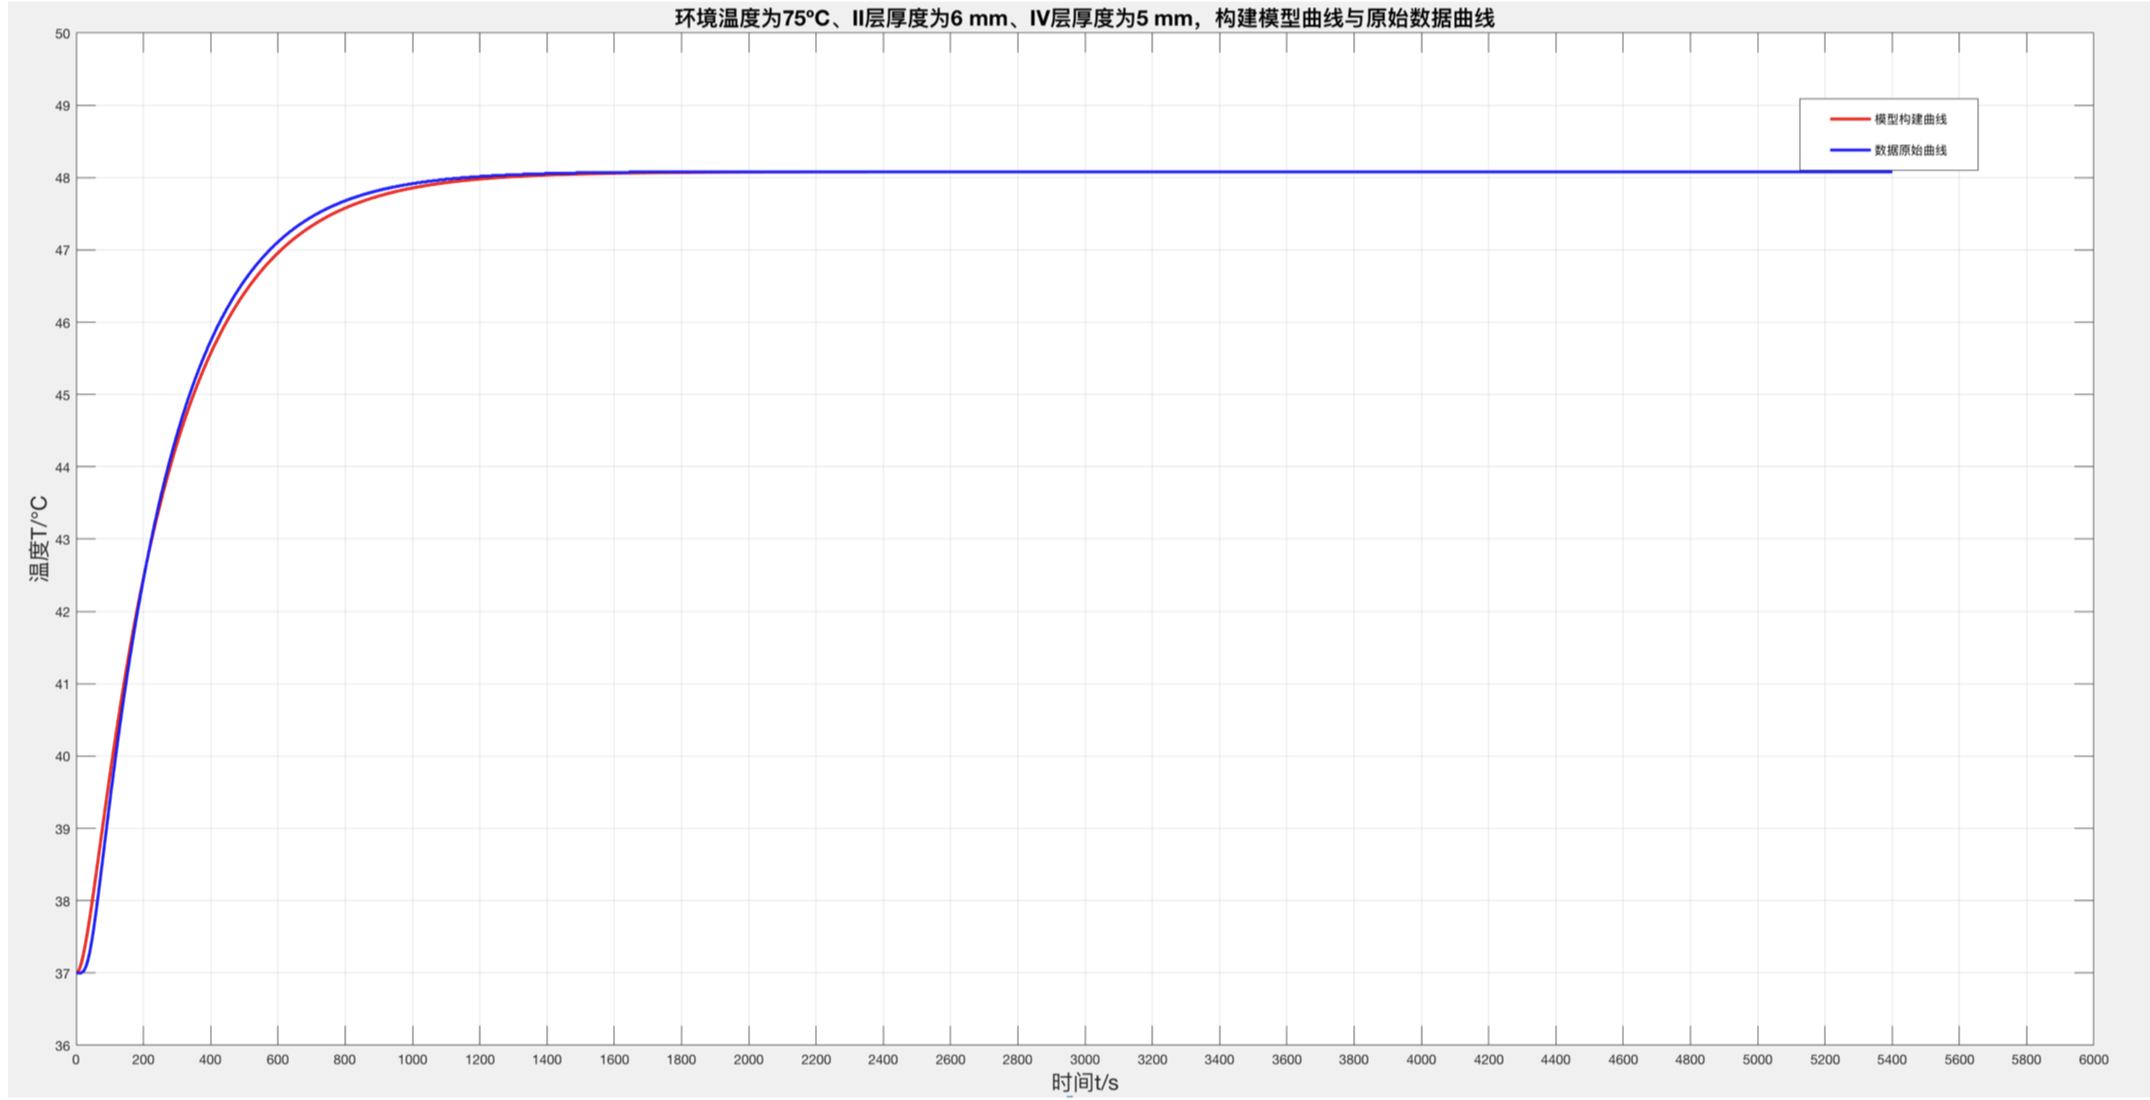
\includegraphics[width=0.7\textwidth]{4.png}
\caption{Curve comparison between the curve obtained by the model and the original data}
% \label{Fig 1}
\end{figure}
\indent From the image, the curve obtained by the model can be roughly approximated by the curve obtained from the original data. We use the difference method to obtain the difference between the model solution data and the original data as shown in the following figure:
\begin{figure}[H]
\centering
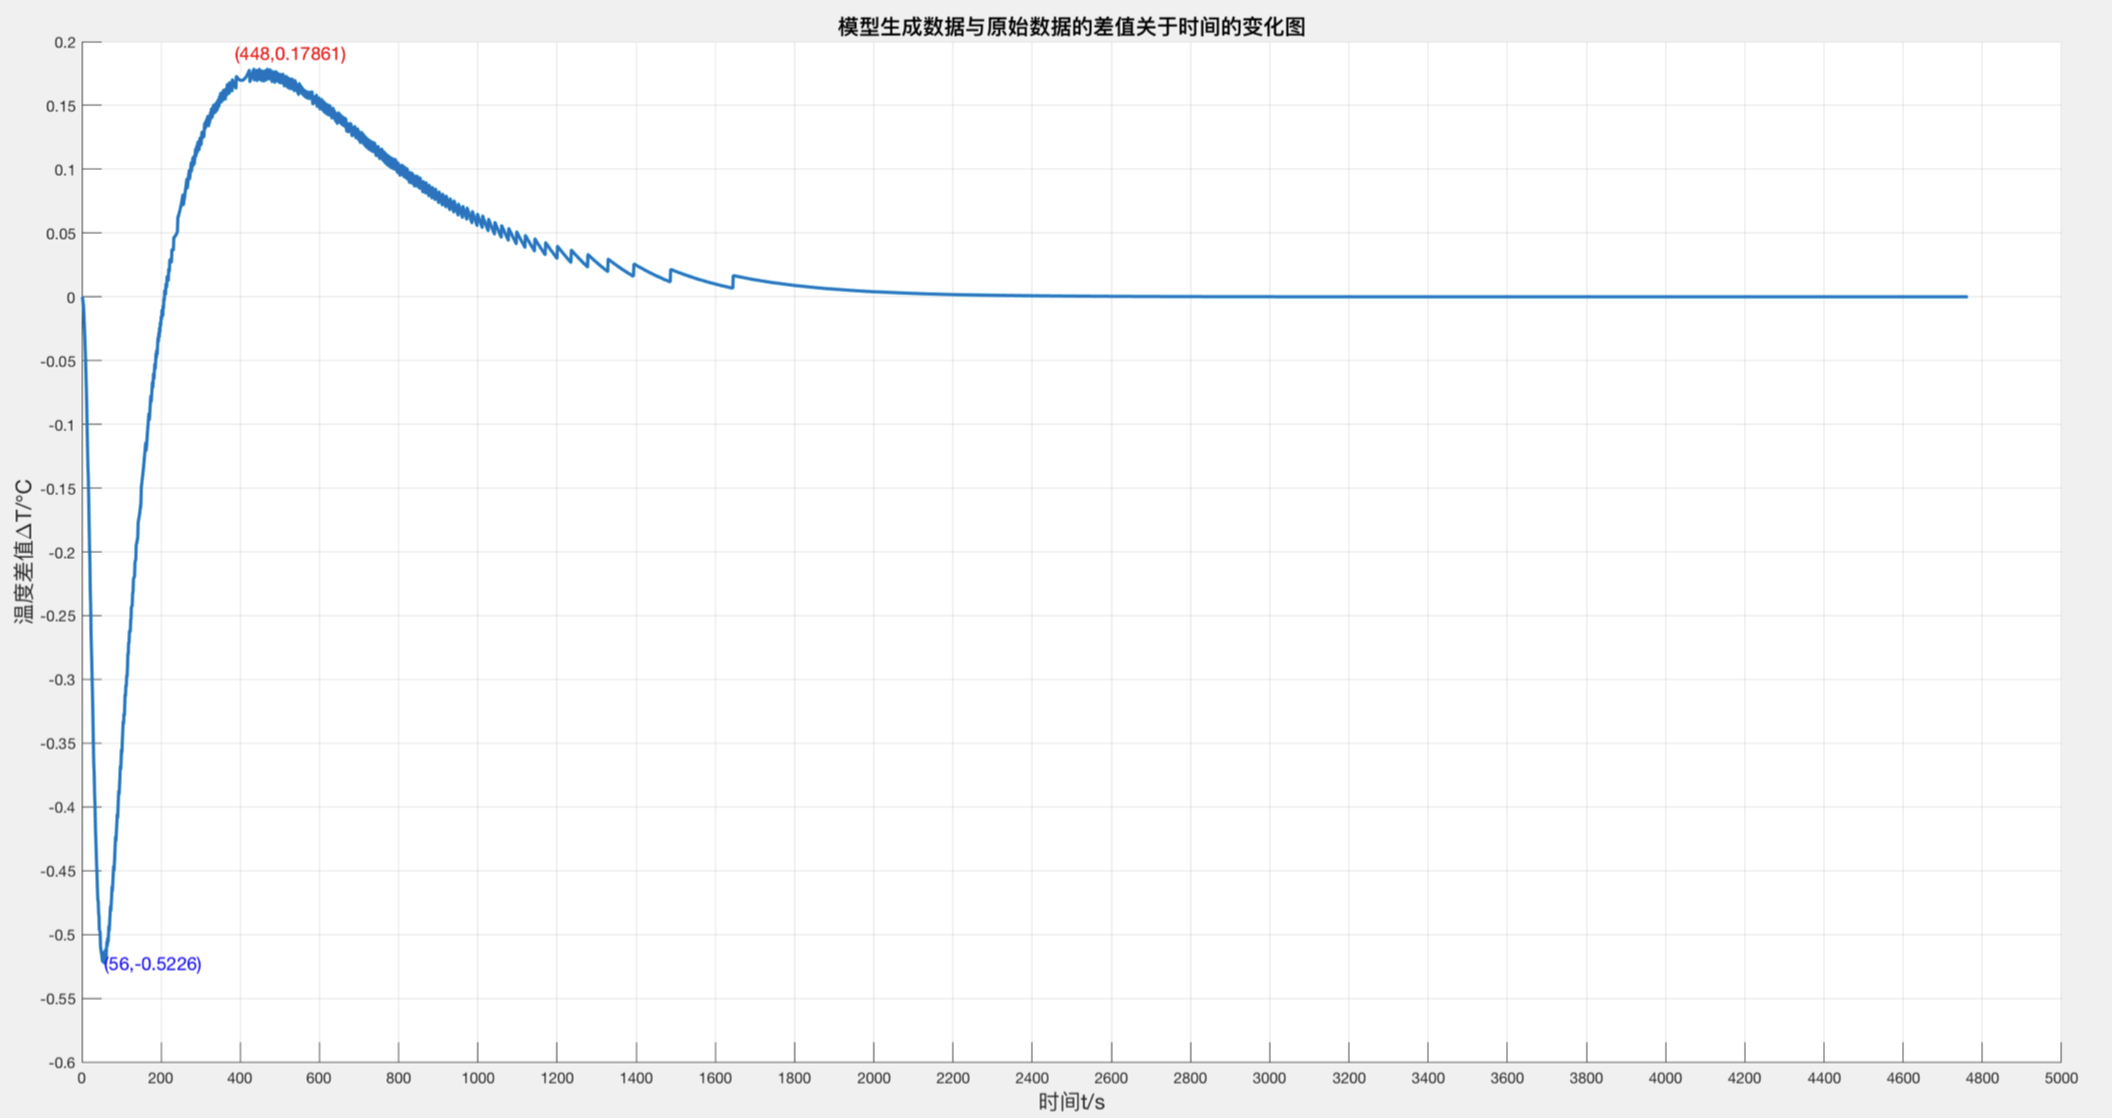
\includegraphics[width=0.7\textwidth]{5.png}
\caption{The model solves the difference between the data and the original data with respect to the image of time $t$}
% \label{Fig 1}
\end{figure}
According to the image and the corresponding function, it can be accurately calculated that when $t = 56s$, the difference between the model solution data and the original data is the largest (that is, the absolute value of the function value is the largest) $|\Delta t| = 0.5226$, and $\exists t_0$ , when $t > t_0$, there is $|\Delta T|$ infinitely close to 0.

\section{Error Analysis}
Modeling Error\cite{taylor1997introduction}: A mathematical model is a model that abstracts a specific problem, ignores secondary factors, and makes reasonable assumptions. Its essence simplifies the actual problem. Therefore, the error that occurs during our simplification of the problem is the model error. In this paper, the model error is expressed in:

1) In the process of mathematical modeling, we only consider the heat transfer caused by the heat transfer method, and ignore the other two forms of heat transfer, namely heat radiation and heat convection.

2) We assume that the temperature inside the same material changes linearly during the establishment of the model. However, in reality, the material may be unevenly distributed, resulting in a nonlinear temperature change inside the material. Our assumptions about the linear change in temperature within the same material may cause the final result to deviate from the actual situation.

Method Error\cite{bevington1993data}: The calculation formula contained in the algorithm is itself an approximate solution (continuous discretization processing, infinite finite processing, etc.), and the error generated is called the method error, also called the truncation error. Truncation Error). In this paper, the method error is expressed in: We use the solution method of the micro-element method to treat the temperature in a micro-element as constant, and consider the heat conduction as the flat-wall heat conduction, so as to solve the problem by using Fourier's law. The heat absorbed by each material layer is derived, and the temperature rise of the material is derived. Although we try to reduce ∆t as much as possible to ensure the accuracy of the model, but due to the accuracy of the computer, we artificially $\Delta t = 0.001$, resulting in a certain deviation between the final result and the actual situation, but this The deviation value is small.

\newpage

\bibliographystyle{plain}
\bibliography{biblist}

\end{document}
